\documentclass[twoside, openany]{report}

\usepackage{lmodern}
\usepackage{xcolor}
\usepackage[utf8]{inputenc}
\usepackage[T1]{fontenc}
\usepackage[francais]{babel}
\usepackage[top=1.5cm, bottom=1.5cm, left=1.5cm, right=1.5cm]{geometry}
\usepackage{wrapfig}
%\usepackage[frenchb]{babel}
%\usepackage{layout}
%\usepackage{setspace}
%\usepackage{soul}
%\usepackage{ulem}
%\usepackage{eurosym}
%\usepackage{bookman}
%\usepackage{charter}
%\usepackage{newcent}
%\usepackage{lmodern}
%\usepackage{mathpazo}
%\usepackage{mathptmx}
%\usepackage{url}
%\usepackage{verbatim}
%\usepackage{moreverb}
%\usepackage{wrapfig}
%\usepackage{amsmath}
%\usepackage{mathrsfs}
%\usepackage{asmthm}
%\usepackage{makeidx}
%\usepackage{tikz} %Vectoriel
\usepackage{wrapfig}
\usepackage{graphicx}
\usepackage{listings}
\usepackage{fancyhdr}
\usepackage{multido}
\usepackage{amssymb}
%\usepackage{sectsty}
%Permet de souligner
\usepackage[normalem]{ulem}
%Permet d'encadrer
\usepackage{fancybox}
%Permet la gestion des hauts et bas de page
\usepackage{fancyhdr}
\definecolor{vert}{rgb}{0.2,0.5,0.2}
\definecolor{orange}{rgb}{0.9, 0.6, 0.35}

\makeatletter
\def\clap#1{\hbox to 0pt{\hss #1\hss}}%
\def\ligne#1{%
	\hbox to \hsize{%
		\vbox{\centering #1}}}%
		\def\haut#1#2#3{%
			\hbox to \hsize{%
				\rlap{\vtop{\raggedright #1}}%
					\hss
					\clap{\vtop{\centering #2}}%
					\hss
					\llap{\vtop{\raggedleft #3}}}}%
					\def\bas#1#2#3{%
						\hbox to \hsize{%
							\rlap{\vbox{\raggedright #1}}%
								\hss
								\clap{\vbox{\centering #2}}%
								\hss
								\llap{\vbox{\raggedleft #3}}}}%
								\def\maketitle{%
									\thispagestyle{empty}\vbox to \vsize{%
										\haut{}{\@blurb}{}
										\vfill
											\vspace{4cm}
										\begin{flushleft}
										\usefont{OT1}{ptm}{m}{n}
										\huge \@title
											\end{flushleft}
										\par
											\hrule height 4pt
											\par
											\begin{flushright}
										\usefont{OT1}{phv}{m}{n}
										\Large \@author 
											\par
											\end{flushright}
											\begin{flushleft}
										\vspace{6cm}
											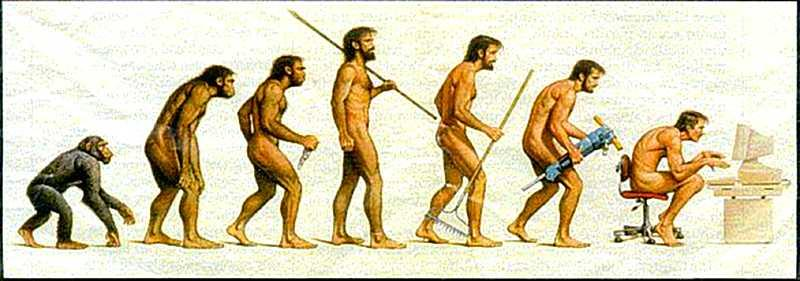
\includegraphics[width=322px]{img_garde2.jpg}
											\end{flushleft}				

										\vspace{1cm}
										\vfill
											\vfill
											\begin{flushleft}
											\vspace{2,8cm}
											Pour Madame Cros~~~~~~~~~~~~~~~~~~
												~~~~~~~~~~~~~~~~~~~~~~~~~~~~~~
											~~~~~~~~~~~~~~~~~~~~~~~~~~~~~~~~~~
											~~~~~~~~~~~~~~~~~~~~~~~~~~~~~~~~~~
											Année 2010-2011
											\end{flushleft}
									}%
									\cleardoublepage
								}
\def\date#1{\def\@date{#1}}
\def\author#1{\def\@author{#1}}
\def\title#1{\def\@title{#1}}
\def\location#1{\def\@location{#1}}
\def\blurb#1{\def\@blurb{#1}}
\date{\today}
\author{}
\title{}
\location{Université Toulouse III}\blurb{}
\makeatother
\title{Les théories de l'évolution}
\author{La religion peut elle cohabiter avec la science?}
\location{Toulouse}
\blurb{%
	\begin{wrapfigure}[19]{l}{0px}
	~~~~~~~~~~~~~	~~~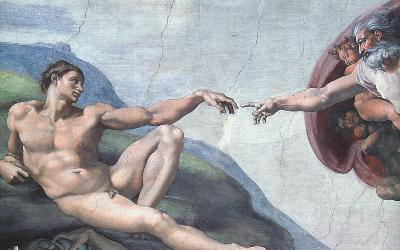
\includegraphics[width=232px]{img_garde1.jpg}
	\end{wrapfigure}
	\begin{flushleft}
			
\includegraphics[width=150px]{logo_ups.png}
			\vspace{1cm}
		 \\\Large{Antoine de \textsc{Roquemaurel} \\Kévin \textsc{Séguy}}\\ 
			 Groupe F
	\end{flushleft}
}% 


\lhead{Les théories de l'évolution}
\rhead{PB: La religion peut elle cohabiter avec la science?}

\lfoot{
\includegraphics[width=40px]{logo_ups_min.png}}
\rfoot{Kévin Séguy \& Antoine de Roquemaurel Groupe F}
\cfoot{\thepage}

\makeatletter
\def\@makechapterhead#1{%

  \vspace*{5\p@}%
  {\parindent \z@ \normalfont \small{
    \interlinepenalty\@M
    \Huge \bfseries\thechapter\quad#1\par\nobreak
    \vskip 5\p@}
  }}
	\newpage
\makeatother

\pagestyle{fancy}
\begin{document}
	\maketitle
	\paragraph{}
	Il était une fois ... Le Monde et l'Homme\\
	La naissance de notre bonne vieille planète bleu
	reste encore flou, beaucoup de personnes se disputent encore la vérité de
	nos jours ainsi que sur la naissance de l'être humain.
	\paragraph{}
	Que se soit les explications \textbf{religieuses} pratiquement semblable, à 
	l'exception du nom des acteurs de la création, ou des explications 
	\textbf{scientifiques}, personne n'est d'accord sur le sujet, mais est ce 
	que tout de même la cohabitation est possible?

\paragraph{}
	Voici la question à laquelle nous allons répondre dans ce 
	dossier culture sans prétention aucune.
	
	\begin{wrapfigure}[19]{l}{250px}
		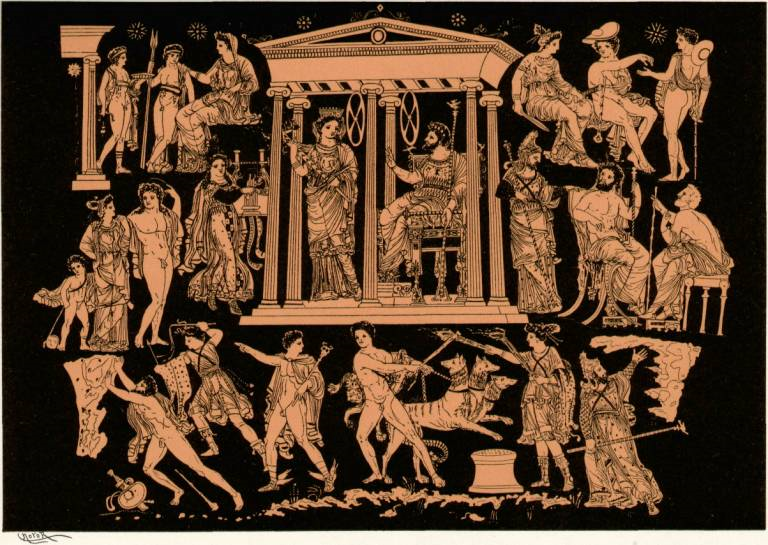
\includegraphics[width=250px]{img1.png}
		\caption{Les dieux de l'olympe}
	\end{wrapfigure}

	Les premières questions se posèrent déjà au temps de l'antiquité Grec
	\footnote{Les Grecs étaient une civilisation fortement évolué}, 
	les philosophes de l'époque était pour la plupart physicien, mathématicien,
	théologien ou poètes 
	\footnote{ces derniers ayant une importance majeur pour la suite}.\\

	Ils sont les détenteurs de toutes les explications de notre 
	monde moderne, mais aussi la source de toutes ces disputes. En effet 
	ces hommes de science cherchaient des réponses sur tous les domaines, 
	essayant d'expliquer pourquoi les choses se passaient ainsi et comment les 
	démontrer, ils ont ainsi inventés sans le savoir ce qui se transformera 
	plus tard en religion.\\
	Ce sont leurs écrits sous forme de poème moralisateur ou d'histoire 
	fantastique\footnote{Théogonie d'Hésiode, les épopées d'Homère} mettant en 
	scène des hommes avec des qualités démesurés, des Héros en somme se battant 
	contre des créatures imaginaires \footnote{créatures qui représentaient les
	choses de la société} envoyés par des forces surpassant de loin l'Homme mais
	qui ne pouvait pas interagir directement sur leurs sujets, ainsi donc la 
	naissance des dieux de l'olympe, d'une religion Polythéiste et de la 
	mythologie Grecque ainsi que Romaine.

\paragraph{}
	Les Hommes croyaient en ces histoires est dévouaient un culte en ces forces
	mystiques \footnote{chaque chose avait un Dieu dédié par exemple Apollon Dieu
	de la Musique et de la Guérison plus tard Dieu Solaire\\}.\\
	Voici le début de l'histoire de la religion, par la suite trois religions 
	Monothéiste on fait leurs apparitions le \textit{Christianisme}, 
	\textit{l'Islam} et le \textit{Judaïsme}, des écrits bien démarqués et 
	officiel existent qui relatent la naissance du Monde jusqu'à la création de
	l'Homme ainsi que la conduite que doit adopter l'humanité (croyante).\\ \\

	\begin{figure}[h]
	\begin{center}
		
\includegraphics[width=200px]{img2.png}
	\end{center}
		\caption{Islam, Christianisme et Judaïsme}
	\end{figure}
	\tableofcontents
	\textcolor{vert}{\part{Explications sur la naissance 
							du monde et de notre univers}}
		\textcolor{orange}{\chapter{De la bible au Big Bang!}}
\section{Hypothèse du big bang}
\paragraph{}
	\begin{wrapfigure}[14]{l}{155px}
	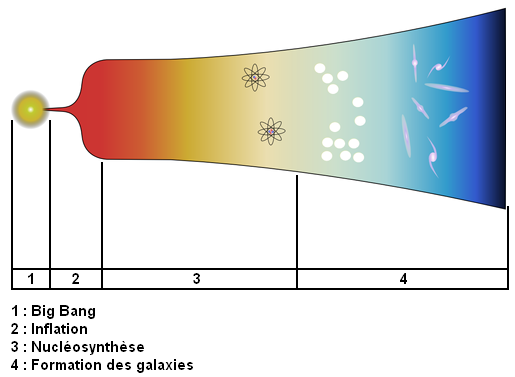
\includegraphics[width=150px]{img3.png}
	\caption{Hypothèse du Big Bang}
\end{wrapfigure}
Comme tout le monde le sait, il existe plusieurs hypothèses sur le sujet, 
et aucune n'est sûr encore de nos jours ce sont des théories. \\
La naissance de l'Univers est sans aucun doute le grand débat cosmologique de ce 
siècle. Deux grandes théories se sont affrontés. Finalement, l'une l'a emporté 
sur l'autre, mais comment les scientifiques ont-ils pu affirmer que l'une était 
correcte contrairement à l'autre ?\\
Ces deux grandes théories ont essayé d'expliquer l'origine de l'Univers. 
La première, la théorie du \textbf{\textsc{Big Bang}}, affirme que l'Univers à 
commencé par une explosion massive en un seul point de l'espace il y a environ 
quinze milliards d'années.\\ \\ \\ \\ \\

Les anciennes religions polythéistes qu'en à elles se rapprochent étrangement de
du Big Bang car tout naitrait du Chaos, celui ci donna naissance à la Terre
\footnote{Représenté par la Déesse Gaia}, qui créa le Ciel, le Temps
\footnote{Représenté par Chronos} ainsi que la Vie et la Mort
\footnote{Représenté par Rhéa et les Titans}, ces derniers procréèrent les 
autres dieux qui représente toutes choses existant dans notre monde et utile 
à l'Univers.

\begin{figure}[h]
	\begin{center}
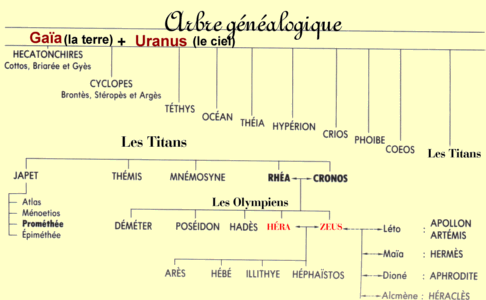
\includegraphics[width=200px]{img4.png}
\caption{Descendance de Gaia}
	\end{center}
\end{figure}

\section{Hypothèse de la création continue}
\paragraph{}
D'après la deuxième théorie, celle de la création continue, il n'y aurait pas eu
de Big Bang. L'univers à toujours existé et existera toujours. Elle envisage un
univers dans lequel les vieilles galaxies ont continuellement disparu au-delà de
l'horizon cosmologique pour être remplacée par de nouvelles galaxies faites de
matière issue du néant. Pour les scientifiques, ces deux théories sont 
invraisemblables, les scientifiques s'intéressant essentiellement 
aux preuves.\\
				  
Si la théorie de la création continue est exacte, l'Univers aurait dû présenter
il y a des millions d'années le même visage qu'aujourd'hui. Or les astronomes 
ont découvert que ce n'était pas le cas, autrefois, les galaxies étaient 
réparties différemment dans l'espace et il y avait plus de quasars
\footnote{Source de rayonnement quasi-stellaire, galaxie lointaine}. 
La théorie de la création continue semble donc inexacte. \\
	   
\section{Hypothèse religieuse}
Cependant cette deuxième théorie peut se raccrocher à une autre vision de la 
naissance du monde dans la religion cette fois ci dites Moderne.\\
Dans une religion, la création apporte une explication du commencement du monde. 
Le monde serait créé par une ou plusieurs divinités. Ces explications ne sont 
pas justifiées, elles sont <<révélées>> autrement dit, les religions demandent 
d'y croire. \\
		
Dans les religions du livre (judaïsme, christianisme et islam), 
 la création est décrite par des chapitres ou des versets des livres saints. \\
Dans la religion hébraïque, la création est décrite dans le livre de la Genèse, 
 qui est le premier livre de la Torah. Dieu aurait créé le monde et la vie en 
 six jours, et se serait reposé le septième. Le récit de la création est 
 similaire dans la religion chrétienne.

\begin{itemize}
\item \textbf{Premier jour:} Création de la terre, puis de la lumière, du jour 
	et de la nuit. \\
\item \textbf{Deuxième jour:} Création du firmament et du ciel. \\
\item \textbf{Troisième jour:} Séparation de l'eau du sec et création de la mer 
	et des continents. Création de la nature, des arbres et des fruits. \\
\item \textbf{Quatrième jour:} Création des étoiles et des saisons. \\
\item \textbf{Cinquième jour:} Création des poissons et des oiseaux, et de la 
	procréation des animaux. \\
\item \textbf{Sixième jour:} Création des animaux domestiques, des reptiles et 
	des serpents. Création du jardin d Éden, du premier homme Adam à son image
	à partir de la poussière, et de la première femme à partir de la côte de 
	l'homme. \\
\item \textbf{Septième jour:} Repos \\
\end{itemize}

Cependant aucun écrit sur l'Univers ni de ce qu'il pouvait exister avant la 
création du monde, c'est pour cela que cette théorie et de plus en plus 
obsolètes de nos jours.

	\begin{figure}[h]
		\begin{center}
	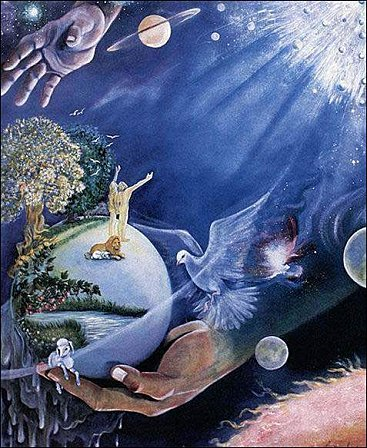
\includegraphics[width=100px]{img5.png}
	\caption{Créationnisme}
		\end{center}
	\end{figure}
	
\textcolor{orange}{\chapter{Confrontation entre la Science et la Religion : 
		Des freins au progrès scientifique ?}}

Avant de commencer... \\
Des préalables pour calmer le débat...\\ 

\paragraph{Les croyants ne sont pas tous créationnistes...}Croire en un Dieu est 
tout à fait compatible avec l'étude des sciences. On peut avoir des croyances et
aussi comprendre le monde qui nous entoure. Le créationniste à une lecture 
littérale des textes religieux, alors que le croyant sait qu'il faut interpréter
les textes.

\paragraph{Les évolutionnistes ne sont pas tous athées...} Cela n'a rien à voir.
L'étude de la nature, de la faune, de l'astronomie et des mécanismes qui les 
régissent n'empêche pas de croire en un Dieu pour, par exemple, donner un sens à
sa vie.

\paragraph{}Croire et comprendre, ou Croire ou comprendre... tel est la 
	question !  \\
Depuis des siècles ce débat fait rage entre la science et la religion notamment
pour l'age du Monde et de l'Univers, les premiers à avoir aborder le sujet étant 
la religio...

\paragraph{Saint Augustin}Admet la date d'environ 5000 ans av. J.-C. pour la 
création de l'Univers\footnote{date donnée à partir de la Genèse}\\
Dernière glaciation, et départ de notre civilisation: environ 10 000 ans av. 
J.-C.

\paragraph{Aristote}Comme la plupart des philosophes grecs, il n'aimait pas 
l'idée de création car elle présentait un arrière-goût d'intervention divine.
\\ Il croyait par conséquent que la race humaine et le monde qui l'entoure 
existaient et existeraient à jamais.

\paragraph{Ussher}
L'archevêque irlandais James Ussher avait déterminé que le monde commençât en
4004 av. J.-C., d'après les Saintes Écritures. 

\begin{itemize}
\item Il étudie la chronologie des patriarches, des juges, des prêtres et des 
	rois. 
\item Il commence par Adam qui est réputé avoir vécu 930 ans et suit les 
	générations. 
\end{itemize}

Publiées en 1650 dans les annales de l'Ancien et du Nouveau Testament, 
les conclusions de Ussher sont très vite acceptées comme définitives par
le clergé.

\paragraph{Buffon}
C'est seulement 150 ans plus tard que Buffon suggère que la Terre pourrait 
avoir 75 000 ans. \\
Il est durement critiqué par l'eglise et doit sous l'autorité du clergé revoir 
ces calculs à la baisse car ils ne correspondent pas au écrit, ce qui emmene 
donc à dire que la religion avait l'autorité sur le savoir et les sciences,
 ce qui laisse à penser que rien n'est exact à cette époque

\paragraph{}
Il faudra encore 50 ans pour que la lecture des couches géologiques renvoie au 
musée les mathématiques généalogiques et théologiques de l'archevêque anglican 
d'Armagh\\
Ce n'est qu au $XX^{éme}$ siécle que les scientiques ne dépendant plus de l'autorité
religieuse commencérent à affirmer que l'Univers daté d'approximativement de 
quinze milliards d'années ce qui ne laissa pas l'Eglise indiferrente, mais
cette fois si impuissante .

	\begin{figure}[h]
		\begin{center}
	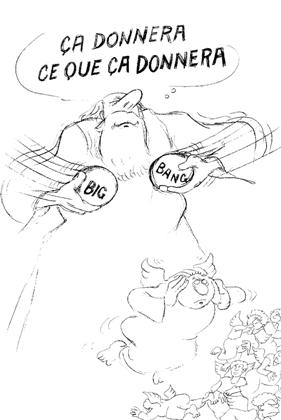
\includegraphics[width=250px]{img6.png}
	\caption{Et Dieu Créa le Big Bang}
		\end{center}
	\end{figure}


	\textcolor{vert}{\part{Les Théories de l'évolution de l'Homme : 
							Lucie ou Adam et Ève ? Peut on les concilier ?}}
		\setcounter{chapter}{0}
\textcolor{orange}{\chapter{La Pomme ou le Singe et ses semblables}}
		\begin{wrapfigure}[20]{l}{80px}
	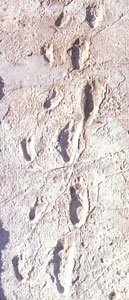
\includegraphics[width=80px]{img7.png}
	\caption{Trace de pas trouvées à Laetoli}
\end{wrapfigure}
\\ \\ \\
	Les traces de pas à Laetoli sont celles d'un homme moderne, c'est la preuve 
	que les hommes n'ont pas évolué et qu'ils ont toujours été présents sur 
	Terre, créés par Dieu.\\ \\
	Petit crédo créationniste qui veut nous faire croire que les hommes et les
	dinosaures ont cohabité !\\ \\  \\

	Plus sérieusement, les traces de pas à Laetoli sont probablement celles d'un 
	australopithèque qui n'est même pas de notre lignée. C'était bien un 
	hominidé bipède qui a marché ce jour-là, mais ce n'est pas un "ancêtre" de 
	l'homme moderne.\\
Les traces de pas de Laetoli ne peuvent pas être celles d'un Homo sapiens, pour 
s'en convaincre il suffit de les comparer visuellement.\\ \\ \\ \\ \\

\section{Les évolutionnistes disent que "l'homme descend du singe"}
\begin{wrapfigure}[13]{r}{110px}
	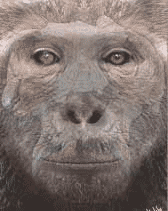
\includegraphics[width=110px]{img8.png}
\end{wrapfigure}
C'est absolument faux, l'homme ne descend pas du singe. C'est un singe lui-même ! 
On attribue, à tort, cette phrase à Charles Darwin et aux scientifiques. 
Ce que l'on sait c'est que les hommes et le chimpanzé ont un ancêtre commun, un 
singe hominoïde. Depuis ce Dernier Ancêtre Commun les espèces se sont séparées
il y a 8 à 9 millions d'années. Les lignées divergentes ont ensuite évolué 
chacune de leur côté. Les gorilles ou les chimpanzés sont donc des cousins 
éloignés de l'homme mais en aucun cas des frères ou des pères!\\ \\
On peut également se poser la question de savoir pourquoi la parenté avec le 
singe est une insulte; Sans doute parce qu'elle rappelle que l'homme est un 
animal parmi d'autres. Ni supérieur, ni inférieur. Cette mise au point gêne 
les extrémistes qui positionnent l'homme au-dessus des autres espèces comme un 
aboutissement. \\
A ce propos il est bon de rappeler que l'histoire de la Terre s'est faite sur 
plusieurs milliards d'années alors qu'Homo sapiens n'apparaît qu'il y a 
seulement 195 000 ans...

\section{La théorie de l'évolution ce n'est qu'une hypothèse}
\begin{wrapfigure}[13]{l}{150px}
	
\includegraphics[width=150px]{img9.png}
\end{wrapfigure}

La biologie avance par hypothèse et théories (comme en chimie, en géologie, en 
génétique). En avançant une hypothèse le scientifique doit vérifier qu'elle 
tient debout, argumenter, trouver des preuves, expérimenter. Un vrai 
scientifique doit accepter que sa théorie soit réfutée, contredite, 
ce n'est pas pour cela qu'elle est fausse ! \\
Sans théorie ni hypothèse nous penserions toujours que la Terre est plate!\\
La théorie de l'évolution est aujourd'hui vérifiée par les faits, les fossiles, 
les expériences. Cela n'empêche pas que des scientifiques puissent continuer 
à travailler le sujet, comme n'importe quelle théorie. \\
Le créationniste, quelle que soit sa religion, ne se base pas sur des faits mais
généralement sur un livre qui présente non pas une théorie mais une histoire. 
Le fait d'être croyant n'empêche d'ailleurs pas de prendre la théorie de 
l'évolution en considération. \textit{Le Pape Jean Paul II a lui même reconnu 
	que la théorie de l'évolution n'était pas qu'une hypothèse}.\\

Depuis 1987, une nouvelle forme de créationnisme voit le jour aux États-Unis, le 
Dessin Intelligent (ou Intelligent Design). Le but avoué est de faire enseigner
le Dessin Intelligent dans les écoles américaines en se parant d'une apparence 
scientifique. Ces partisans remplacent la notion de Dieu par celle de l'être 
supérieur pour expliquer que l'harmonie de notre monde ne peut s'expliquer que 
par une intervention extérieure, c'est-à-dire divine !	
	\begin{figure}[h]
		\begin{center}
	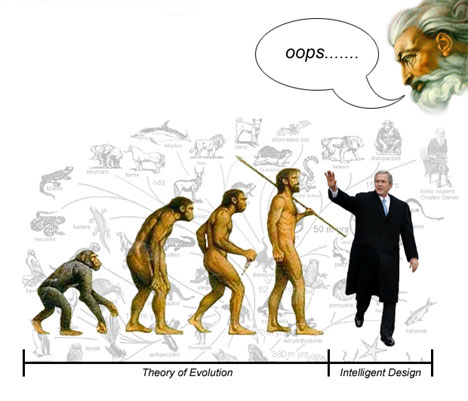
\includegraphics[width=250px]{img10.png}
	\caption{Théorie de l'évolution}
		\end{center}
	\end{figure}	
	
\textcolor{orange}{\chapter{Une lecture nouvelle de théories religieuses}}
Depuis quelques temps, les hommes d'église nous propose une nouvelle façon 
d'aborder les écrits religieux, Pie XII (pape de 1939 à 1958), Jean Paul II 
(pape de 1978 à 2005) longuement critiqué à ce sujet notamment par les 
Créationnistes, ils ont été les prédécesseurs de ce mouvement de lecture nouvelle.
Plusieurs ouvrages également ont été édité comme "Une Nouvelle Lecture Biblique"
de Simon Hazan et Antoine Mercier (édité chez Lichma en 2010), 
"Divine Chamaillerie" de Sébastien Allali (édité chez Lichma en 2010).\\
Mais tout cela est une question d'interprétation, nous allons pour rester dans 
notre sujet  prendre et expliquer certains passages et certaines images qui se 
lie le plus avec la Science.\\
Tout d'abord, la création du monde, précédemment nous l'estimions à quinze milliards
d'années et la Bible en sept jours or partons du principe qu'un jour ne soit pas un
jour réel mais un jour Divin prenons le $6^{éme}$ jours création des animaux 
domestiques, des reptiles et des serpents, du premier homme et la femme toutes
ces choses là sont dans un stade final au niveau de l'évolution  et si chaque 
jour divin représentait un à deux milliards d'années plutôt surprenant car cela 
colle exactement aux estimations des scientifiques à cette étape 
d'évolution et rajoutons maintenant les six autres jours divins, nous arrivons à
un total de sept à quatorze milliards d'années ! 
Cela ne vous rappelle rien? Une fois de plus une hypothèse qui se
laisse imaginer.\\ \\

\begin{wrapfigure}[9]{r}{110px}
	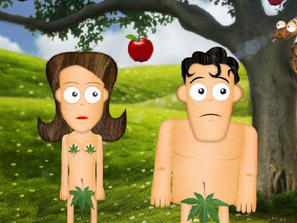
\includegraphics[width=110px]{img11.png}
\end{wrapfigure}
Si nous continuons avec Adam et Ève (s'ils ont existé) leurs ages étaient estimé 
à 930 ans ce qui peut paraitre aberrant et impossible, cependant si nous partons 
du principe une nouvelle fois que cette age fut compté en mois cela ne ferait 
plus que soixante-dix sept ans. \\
Un peu plus crédible ?\\
Terminons avec le Jardin d Éden et l'arbre Sacré, lieu où vivaient Adam et Ève
immortel à la condition qu'ils étaient défendu de croquer la moindre pomme sous 
peine d'être exclu d Éden (tout comme Satan).\\
L'image que nous pouvons faire du Jardin d Éden et de l'immortalité qu'elle 
regorgeait ne serait pas lié directement à Adam et Ève mais à l'Humanité 
autrement dit la fécondité, s'ils se reproduisent et que chaque générations 
fait de même nous trouvons ici une sorte d'immortalité de la race humaine.\\
L'arbre quant à lui referme la nature de l'Homme, le fait de prendre une pomme 
montre qu'il veut toujours plus que ce qu'il n'a, le confort, toujours plus 
de savoir, toujours plus d'évolution et de technologie, le matérialisme, la 
conquête et la recherche de la supériorité ... \\Tout cela sans se soucier du mal
qui l'engendre et de la détérioration d'autrui et de son monde.



		\newpage
		\vfill
		\vspace{6cm}
Pour conclure ce dossier culture sur La Théorie de L'évolution : La Religion peut 
elle cohabiter avec la Science ?\\
Je donnerais une réponse positive comme nous avons essayé de le montrer tout au 
long du dossier.\\ 
Pour cela, il ne faut pas lire les écrits religieux à la lettre mais bien entre
les lignes, tous les religieux ne sont pas Créationniste et certains scientifique
sont croyants ce qui prouve bel et bien une certaine harmonie entre ces deux 
mondes.\\ \\ \\

Exemple concret de la chose , une personne célèbre tant dans le monde religieux 
que dans la science je vous parle ici de Monsieur Georges lemaître, prêtre, 
astrophysicien et mathématicien belge.\\ 
L'abbé Lemaître est alors reconnu comme le précurseur de la théorie de 
l'expansion de l'univers. Élu membre de l'Académie pontificale des Sciences lors
de sa création en 1936, il en deviendra le Président en 1960 et le restera 
jusqu'à sa mort en 1966. \\ \\ \\ \\

Nos sources sont variées tout d'abord, Internet (wikipédia), les écrits de Darwin 
et Lamarck, reportage sur France 5 de Steven Hawking, certains passages de la Genèse.
		\vfill

\end{document}
